% @file   thesis.tex
% @brief  graduation thesis of Shibaura Institute of Technology
% @author Kataoka Nagi al18036[at]shibaura-it.ac.jp
% @date   2021-12-21 15:19:48
% $Version:   1.0
% @parHistory
% add
% Copyright (c) 2021 Kataoka Nagi

\documentclass[12pt,a4j]{jreport}
\setcounter{secnumdepth}{5}
\usepackage[dvipdfmx]{graphicx}
\usepackage{amsmath,amssymb}
\usepackage{comment}
\usepackage{graphicx}
\usepackage{here}
\usepackage{bm}
\usepackage{url}

\renewcommand{\baselinestretch}{1.5}

\renewcommand{\bibname}{参考文献}





\begin{document}


%%%%%%%%%%%%%%%%%%%%%%%%%%%%%%%%%%%%%
% 表紙
%%%%%%%%%%%%%%%%%%%%%%%%%%%%%%%%%%%%%
\begin{titlepage}

\begin{center}

\vspace*{2cm}
\Large 2021 年度 芝浦工業大学 工学部 情報工学科\\

\vspace*{1.0cm}
\Huge 卒 \qquad 業 \qquad 論 \qquad 文\\
\vspace*{2.5cm}

\Large 記事トピックのクラスタを用いた\\多言語ニュース推薦手法の提案

\vspace{4cm}
\begin{tabular}{ll}
\vspace*{2mm}
学籍番号 & \qquad $\mathbf{AL18036}$ \\
\vspace*{2mm}
氏\phantom{  }名 & \qquad 片岡 \quad 凪   \\
\vspace*{2mm}
指導教員   & \qquad 木村 \quad 昌臣
\end{tabular}
\end{center}
\end{titlepage}



% \begin{abstract}
% このファイルは,情報工学科卒業論文の推奨テンプレートである.概要書とは異なり,卒業論文本体のテンプレートはあくまで推奨であるので,このテンプレートを下にして文字サイズや行間などを修正したものを利用しても良く,またこのテンプレートを使わなくても良い.

% この部分の研究概要では,研究背景,解決したい問題,研究目的,提案手法,評価方法,評価の結果について簡潔に書く.
% 概要の有無は任意.
% \end{abstract}


{\makeatletter
\let\ps@jpl@in\ps@empty
\makeatother
\pagestyle{empty}
\tableofcontents
\clearpage}

\setcounter{page}{1} 
\pagestyle{plain}

%%%%%%%%%%%%%%%%%%%%%%%%%%%%%%%%%%%%%%%%%%%%%%%%%%%%%%%%%%%%
% 書式 
%%%%%%%%%%%%%%%%%%%%%%%%%%%%%%%%%%%%%%%%%%%%%%%%%%%%%%%%%%%%
% 図の参照『図\ref{fig_nn}に3層のニューラルネットワークを示す』
% \begin{figure}[ht]
% 	\centering
% 	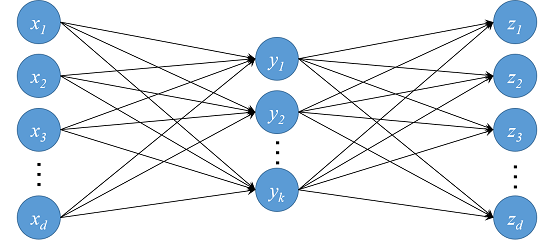
\includegraphics[keepaspectratio, width=120mm]{img/sample.png}
% 	\caption{提案法に用いた3層のニューラルネットワーク.キャプションにはこの図の説明を書く.}
% 	\label{fig_nn}
% \end{figure}

% 表の参照『表\ref{table_a}に手法Aおよび手法Bの正答率を示す』
% \begin{table}[ht]
%   \caption{手法Aおよび手法Bの正解率と平均計算時間.}
%   \label{table_a}
%   \centering
%   \begin{tabular}{lcr}
% \hline
% 手法   & 正解率[\%]  &  計算時間[ms]  \\
% \hline \hline
% 手法A  & 92.3  & 512 \\
% 手法B  & 87.4  & 32  \\
% \hline
%   \end{tabular}
% \end{table}

% 参考文献『井尻らは,X線CTとデジタルカメラを用いた3次元モデリング法を提案した\cite{Ijiri18}.』
% 参考文献リスト『著者1, 著者2,...,著者N. タイトル. 論文誌or学会名, 巻, 号, ページ, 発表年. 』
% Webページ『著者. ページタイトル. ページURL(2021年7月31日参照).』


%%%%%%%%%%%%%%%%%%%%%%%%%%%%%%%%%%%%%%%%%%%%%%%%%%%%%%%%%%%%
\chapter{序論}
%%%%%%%%%%%%%%%%%%%%%%%%%%%%%%%%%%%%%%%%%%%%%%%%%%%%%%%%%%%%

(用紙や文字のなどのサイズには井尻先生のTeXテンプレートをそのまま利用しています)

%%%%%%%%%%%%%%%%%%%%%%%%%%%%%%
\section{研究背景}
~
% @see 

%%%%%%%%%%%%%%%%%%%%%%%%%%%%%%
\section{研究目的}
~
% @see 

%%%%%%%%%%%%%%%%%%%%%%%%%%%%%%
\section{本論文の構成}
~
% @see 

%%%%%%%%%%%%%%%%%%%%%%%%%%%%%%%%%%%%%%%%%%%%%%%%%%%%%%%%%%%%
\chapter{本研究で用いる知識と技術}
%%%%%%%%%%%%%%%%%%%%%%%%%%%%%%%%%%%%%%%%%%%%%%%%%%%%%%%%%%%%


%%%%%%%%%%%%%%%%%%%%%%%%%%%%%%
\section{ニュース推薦システム}
多くのWebニュースサイトでは,様々なアルゴリズムを用いて読者の趣向に合わせた記事が提示されている.
アルゴリズムの例として,
読者が閲覧した記事に似た記事を推薦するコンテンツベースフィルタリング(Content-Based Filtering)や
似た趣向を持つ他の読者の閲覧記事を推薦する協調フィルタリング(Collaborative Filtering),
この2つや他のルールを併用したハイブリッドな手法などがある\cite{karimi_news_2018}.
このような読者にパーソナライズした推薦アルゴリズムをニュース推薦システム(News Recommender Systems)という.
アルゴリズムの評価指標には,記事の閲覧回数,閲覧記事のカテゴリ,読者の位置情報,他サイトの閲覧履歴や購買情報などがある.
% @see News recommender systems – Survey and roads ahead

%%%%%%%%%%%%%%%%%%%%%%%%%%%%%%
\section{ニュース推薦システムが生むバイアス}
~
% @see 0517-

\subsection{エコーチェンバー問題}
~
% @see 

\subsection{フィルターバブル問題}
~
% @see 

%%%%%%%%%%%%%%%%%%%%%%%%%%%%%%
\section{機械学習}
~
% @see 

\subsection{ニューラルネットワーク}
~
% @see 

\subsection{教師あり学習}
~
% @see 

\subsection{Attention(LSTMに触れる)}
~
% @see 

\subsection{Transformer(教師あり分類にも触れる)}
~
% @see 

\subsection{BERT}
~
% @see 

\subsection{RoBERTa(BERTとの比較など)}
~
% @see 

%%%%%%%%%%%%%%%%%%%%%%%%%%%%%%
\section{文章分類}
~
% @see 

\subsection{テキストの前処理}
~
% @see 

\subsection{単語埋め込み}
~
% @see 

\subsection{Transformer分類器}
~
% @see 

\subsection{分類モデルの評価(acc, prcなどの議論)}
~
% @see 

%%%%%%%%%%%%%%%%%%%%%%%%%%%%%%
\section{文章の類似度の算出}
~
% @see 

\subsection{Sentence-BERT}
~
% @see 

\subsection{コサイン類似度}
~
% @see 

%%%%%%%%%%%%%%%%%%%%%%%%%%%%%%
\section{クラスタリング}
~
% @see 

\subsection{非階層クラスタリング}
~
% @see 

\subsection{階層的クラスタリング}
~
% @see 

\subsection{Ward法}
~
% @see 

\subsection{(その他使用した手法)}
~
% @see 

\subsection{t-SNE (使うかも)}
~
% @see 


%%%%%%%%%%%%%%%%%%%%%%%%%%%%%%%%%%%%%%%%%%%%%%%%%%%%%%%%%%%%
\chapter{関連研究}
%%%%%%%%%%%%%%%%%%%%%%%%%%%%%%%%%%%%%%%%%%%%%%%%%%%%%%%%%%%%


%%%%%%%%%%%%%%%%%%%%%%%%%%%%%%
\section{ニュース推薦システムのバイアスの解決}
~
% @see 

\subsection{Breaking the filter bubble: democracy and design}
~
% @see 

\subsubsection{(UIでバブルの可視化)(結局表示されるものにバイアスがかかる,行動に繋がらない)}
~
% @see 

\subsubsection{(トピックモデル,LSI, LDAの議論)}
~
% @see 

%%%%%%%%%%%%%%%%%%%%%%%%%%%%%%
\section{話題の定量化によるニュース推薦手法}
~
% @see 

\subsection{トピックマップ}
~
% @see 

\subsection{Labeled Bilingual Topic Model for Cross-Lingual Text Classification and Label Recommendation}
~
% @see 

\subsubsection{(LDAの利用)}
~
% @see 

%%%%%%%%%%
% \section{LSI}
~
% @see 

%%%%%%%%%%%%%%%%%%%%%%%%%%%%%%
\section{(要追加調査:比較評価できる推薦手法)(出来事,主張に着目するシステムなど)}
~
% @see 

\subsection{Investigating COVID-19 News Across Four Nations A Topic Modeling and Sentiment Analysis Approach}
~
% @see 

\subsubsection{トピックモデル,top2vec, roberta}
~
% @see 

%%%%%%%%%%
% \section{tf-idf -->}
~%% @see 
 <!-- SCDV -->


%%%%%%%%%%%%%%%%%%%%%%%%%%%%%%%%%%%%%%%%%%%%%%%%%%%%%%%%%%%%
\chapter{提案手法}
%%%%%%%%%%%%%%%%%%%%%%%%%%%%%%%%%%%%%%%%%%%%%%%%%%%%%%%%%%%%


%%%%%%%%%%%%%%%%%%%%%%%%%%%%%%
\section{使用する語彙と基準の定義}
~
% @see 

\subsection{文と文章}
~
% @see 

\subsection{出来事の文}
~
% @see 

\subsection{主張の文}
~
% @see 

\subsection{文が示す話題の類似度}
~
% @see 

%%%%%%%%%%%%%%%%%%%%%%%%%%%%%%
\section{記事の出来事と主張のクラスタを用いた多言語ニュース推薦}
~
% @see 

\subsection{手法概要}
~
% @see 

\subsection{クラスタリングの順序の検討}
~
% @see 

\subsection{(その他報告会などで議論したこと)}
~
% @see 

%%%%%%%%%%%%%%%%%%%%%%%%%%%%%%
\section{データセットの選定}
~
% @see 

\subsection{出来事の文と主張の文の分類器の学習データ(IBM Debater Datasetの議論)}
~
% @see 

\subsection{分類とクラスタリングを行うデータ(covid-19-articlesの議論)}
~
% @see 

%%%%%%%%%%<!-- 
% \section{Japanese fakenews dataset -->}
~
% @see 

%%%%%%%%%%%%%%%%%%%%%%%%%%%%%%
\section{データの前処理}
~
% @see 

\subsection{自然言語処理のためのテキストの前処理(前処理の種類,なぜ前処理するのかなどの議論)}
~
% @see 

\subsection{(その他工夫した前処理)}
~
% @see 


%%%%%%%%%%%%%%%%%%%%%%%%%%%%%%%%%%%%%%%%%%%%%%%%%%%%%%%%%%%%
\chapter{実装}
%%%%%%%%%%%%%%%%%%%%%%%%%%%%%%%%%%%%%%%%%%%%%%%%%%%%%%%%%%%%


%%%%%%%%%%%%%%%%%%%%%%%%%%%%%%
\section{システムの設計指針(入出力,使い方など)}
~
% @see 

%%%%%%%%%%%%%%%%%%%%%%%%%%%%%%
\section{システム構成(モジュールの説明)}
~
% @see 

%%%%%%%%%%%%%%%%%%%%%%%%%%%%%%
\section{実装環境(PCスペック,ライブラリバージョンなど)}
~
% @see 

%%%%%%%%%%%%%%%%%%%%%%%%%%%%%%
\section{データの前処理}
~
% @see 

\subsection{正規表現による前処理(awkの正規表現などの議論)}
~
% @see 

\subsection{省略のピリオドに注意した文章の分割(Stanza, spacyの議論)}
~
% @see 

%%%%%%%%%%%%%%%%%%%%%%%%%%%%%%
\section{出来事の文と主張の文の分類}
~
% @see 

\subsection{Simple Transformers}
~
% @see 

%%%%%%%%%%%%%%%%%%%%%%%%%%%%%%
\section{出来事の文章のクラスタリング}
~
% @see 

\subsection{(要検討)}
~
% @see 

%%%%%%%%%%%%%%%%%%%%%%%%%%%%%%
\section{主張の文のクラスタリング}
~
% @see 

\subsection{(要検討)}
~
% @see 


%%%%%%%%%%%%%%%%%%%%%%%%%%%%%% 
% \section{仮説}
~%% @see 
 評価実験を設計するにあたり以下3件の仮説を立てる.
% \begin{itemize}
%   \item 仮説1) .
%   \item 仮説2) 
%   \item 仮説3) 
% \end{itemize}
% この3件の仮設は,それぞれ以下の考察に基づき設定されている.
% 仮説1は...


%%%%%%%%%%%%%%%%%%%%%%%%%%%%%%%%%%%%%%%%%%%%%%%%%%%%%%%%%%%%
\chapter{実験}
%%%%%%%%%%%%%%%%%%%%%%%%%%%%%%%%%%%%%%%%%%%%%%%%%%%%%%%%%%%%


%%%%%%%%%%%%%%%%%%%%%%%%%%%%%%
\section{出来事の文と主張の文の分類}
~
% @see 

\subsection{実験方法}
~
% @see 

\subsection{実験結果}
~
% @see 

\subsection{実験の考察}
~
% @see 

\subsection{(試行錯誤)}
~
% @see 

%%%%%%%%%%%%%%%%%%%%%%%%%%%%%%
\section{出来事の文章のクラスタリング}
~
% @see 

\subsection{実験方法}
~
% @see 

\subsection{実験結果}
~
% @see 

\subsection{実験の考察}
~
% @see 

\subsection{(試行錯誤)}
~
% @see 

%%%%%%%%%%%%%%%%%%%%%%%%%%%%%%
\section{主張の文のクラスタリング}
~
% @see 

\subsection{実験方法(クラスタの階層の基準ごとの評価)}
~
% @see 

\subsection{実験結果}
~
% @see 

\subsection{実験の考察}
~
% @see 

\subsection{(試行錯誤)}
~
% @see 

%%%%%%%%%%%%%%%%%%%%%%%%%%%%%%
\section{(他の研究との比較実験)}
~
% @see 

\subsection{実験方法}
~
% @see 

\subsection{実験結果}
~
% @see 

\subsection{実験の考察}
~
% @see 

\subsection{(試行錯誤)}
~
% @see 


%%%%%%%%%%%%%%%%%%%%%%%%%%%%%%%%%%%%%%%%%%%%%%%%%%%%%%%%%%%%
\chapter{結果と考察}
%%%%%%%%%%%%%%%%%%%%%%%%%%%%%%%%%%%%%%%%%%%%%%%%%%%%%%%%%%%%


%%%%%%%%%%%%%%%%%%%%%%%%%%%%%%
\section{既存手法との比較}
~
% @see 

%%%%%%%%%%%%%%%%%%%%%%%%%%%%%%
\section{提案手法の妥当性}
~
% @see 

\subsection{入力と出力の妥当性}
~
% @see 

\subsection{処理速度の妥当性(分散システムの議論も)}
~
% @see 

%%%%%%%%%%%%%%%%%%%%%%%%%%%%%%
\section{(結果を基に検討)}
~
% @see 

%%%%%%%%%%%%%%%%%%%%%%%%%%%%%%%%%%%%%%%%%%%%%%%%%%%%%%%%%%%%
\chapter{まとめと展望}
%%%%%%%%%%%%%%%%%%%%%%%%%%%%%%%%%%%%%%%%%%%%%%%%%%%%%%%%%%%%


%%%%%%%%%%%%%%%%%%%%%%%%%%%%%%
\section{まとめ}
~
% @see 

%%%%%%%%%%%%%%%%%%%%%%%%%%%%%%
\section{今後の展望}
~%% @see 
 \section{データセットの相性(ディベートとニュース)}
~
% @see 

%%%%%%%%%%%%%%%%%%%%%%%%%%%%%%%%%%%%%%%%%%%%%%%%%%%%%%%%%%%%
\chapter*{謝辞}
\addcontentsline{toc}{chapter}{謝辞}
%%%%%%%%%%%%%%%%%%%%%%%%%%%%%%%%%%%%%%%%%%%%%%%%%%%%%%%%%%%%


%%%%%%%%%%%%%%%%%%%%%%%%%%%%%%%%%%%%%%%%%%%%%%%%%%%%%%%%%%%%
\bibliographystyle{junsrt}
\bibliography{ref.bib}
%%%%%%%%%%%%%%%%%%%%%%%%%%%%%%%%%%%%%%%%%%%%%%%%%%%%%%%%%%%%

\end{document}
